\chapter{User Documentation}

The demo version of our game is called \enquote{Project Nitrogen}, and it is available in the attachments as the folder \emph{Build}.
This is a build for a personal computer with the \emph{Windows} operating system.
In this chapter, we will give instructions on how to run the game, how to navigate its menus, and we provide some reference tables with information the player might find useful.

\section{Instructions}

The attachment folder \emph{Build} contains a few application binaries, a dynamically linked library and directories with the game's assets.
To run the game, simply run the \mono{ProjectNitrogen.exe} binary.

The game will show a \enquote{Made with Unity} splash screen and take you to the main menu.
The main menu contains three large buttons: \enquote{Start}, \enquote{Custom Run} and  \enquote{Exit}.
To start a new run, click the \enquote{Start} button.
The \enquote{Custom Run} button will take you to the run settings screen, and the \enquote{Exit} button will exit the game.

The run settings screen lets you set the seed of the run, and it lets you choose to select the starting blueprints at the start of the run.
To start the run with these settings, press the \enquote{Start} button.
The \enquote{Replay Tutorial} button will disregard these settings, and start a tutorial run instead.
To return to the main menu, press the \enquote{Back} button.

The first run started from the main menu will include the in-game tutorial, which explains how to play the game in an interactive manner.
It explains the goals of the game and the game's controls.

\section{Reference Tables}

In this section, we provide some tables the players might find useful.
The in-game tutorial explains how to control the game, but table~\ref{tab:controls} contains all controls and hotkeys the player can use during battle for reference.
Some hotkeys are not mentioned in the game, but they are not necessary to play it.

We also provide reference tables with all the attackers and blueprints the game contains.
Attackers are in tables~\ref{tab:attackers1} and~\ref{tab:attackers2}.
Blueprints are separated by type:
\begin{itemize}
    \item Economic buildings~--- table~\ref{tab:economic-buildings}.
    \item Special buildings~--- table~\ref{tab:special-buildings}.
    \item Tower~--- tables~\ref{tab:towers1} and~\ref{tab:towers2}.
    \item Abilities~--- table~\ref{tab:abilities}.
\end{itemize}

\begin{table}[H]
    \centering
    \begin{tabular}{m{0.2\textwidth}m{0.7\textwidth}}
        \toprule
        \textbf{Button}                                   & \textbf{Actions}                                                     \\
        \midrule
        \textbf{Left click}                               & Press a user interface button. \vspace{4pt}\newline
        Select a tile, building or attacker in the world, or a blueprint from the blueprint menu. \vspace{4pt}\newline
        Deselect currently selected object (except for a blueprint) and hide the info panel by clicking on empty space.          \\\midrule
        \textbf{Right click}                              & Deselect currently selected object and hide the info panel.          \\\midrule
        \textbf{Right click \newline drag}                & Move the camera.                                                     \\\midrule
        \textbf{Scrolling}                                & Zoom the camera in or out.                                           \\\midrule
        \textbf{Scroll wheel \newline drag}               & Rotate the camera to the left or right.                              \\\midrule
        \textbf{Escape}                                   & Deselect currently selected object and hide the info panel.          \\\midrule
        \textbf{Space}                                    & Start the next wave.                                                 \\\midrule
        \textbf{1} to \textbf{9}                          & Select the 1st to 9th blueprint from the blueprint menu.             \\\midrule
        \textbf{R}                                        & Rotate the currently selected blueprint, if possible.                \\\midrule
        \textbf{W} / \textbf{S} / \textbf{A} / \textbf{D} & Move the camera forward / back / left / right.                       \\\midrule
        \textbf{T} / \textbf{G}                           & Zoom the camera in / out.                                            \\\midrule
        \textbf{Q} / \textbf{E}                           & Rotate the camera left / right.                                      \\\midrule
        \textbf{Tab}                                      & Change the targeting priority of the selected tower to the next.     \\\midrule
        \textbf{Ctrl} + \textbf{Tab}                      & Change the targeting priority of the selected tower to the previous. \\\midrule
        \textbf{Delete}                                   & Delete the selected building.                                        \\\midrule
        \textbf{M}                                        & Mute or unmute the game sounds.                                      \\
        \bottomrule
    \end{tabular}
    \caption{The controls and hotkeys the player can use during a battle.}
    \label{tab:controls}
\end{table}


\begin{table}[H]
    \centering
    \begin{tabular}{m{9mm}m{25mm}D{.}{.}{-1}rm{0.48\textwidth}}
        \toprule
        \textbf{Icon}                                                                 & \textbf{Name}                          & \mc{\textbf{Speed}} & \mc{\textbf{HP}} & \textbf{Description}                                                                                                                                \\
        \midrule
        
\includegraphics[height=7mm]{img/Icons/Attackers/Red Slime.png}               & \footnotesize{Red Slime}               & 1                   & 5                &                                                                                                                                                     \\
        
\includegraphics[height=7mm]{img/Icons/Attackers/Blue Slime.png}              & \footnotesize{Blue Slime}              & 1.4                 & 10               & \footnotesize{When killed, spawns a \emph{Red Slime}.}                                                                                              \\
        
\includegraphics[height=7mm]{img/Icons/Attackers/Green Slime.png}             & \footnotesize{Green Slime}             & 1.8                 & 15               & \footnotesize{When killed, spawns a \emph{Blue Slime}.}                                                                                             \\
        
\includegraphics[height=7mm]{img/Icons/Attackers/Yellow Slime.png}            & \footnotesize{Yellow Slime}            & 3.2                 & 20               & \footnotesize{When killed, spawns a \emph{Green Slime}.}                                                                                            \\
        
\includegraphics[height=7mm]{img/Icons/Attackers/Pink Slime.png}              & \footnotesize{Pink Slime}              & 3.5                 & 25               & \footnotesize{When killed, spawns a \emph{Yellow Slime}.}                                                                                           \\
        
\includegraphics[height=7mm]{img/Icons/Attackers/Black Slime.png}             & \footnotesize{Black Slime}             & 1.8                 & 30               & \footnotesize{Immune to \emph{Explosive} damage. \newline When killed, spawns two \emph{Pink Slimes}.}                                              \\
        
\includegraphics[height=7mm]{img/Icons/Attackers/Lead Slime.png}              & \footnotesize{Lead Slime}              & 1                   & 35               & \footnotesize{Immune to \emph{Physical} damage. \newline When killed, spawns two \emph{Black Slimes}.}                                              \\
        
\includegraphics[height=7mm]{img/Icons/Attackers/Skeleton.png}                & \footnotesize{Skeleton}                & 1.6                 & 20               &                                                                                                                                                     \\
        
\includegraphics[height=7mm]{img/Icons/Attackers/Yellow Skeleton.png}         & \footnotesize{Yellow Skeleton}         & 1.6                 & 60               &                                                                                                                                                     \\
        
\includegraphics[height=7mm]{img/Icons/Attackers/Black Skeleton.png}          & \footnotesize{Black Skeleton}          & 1.6                 & 180              &                                                                                                                                                     \\
        
\includegraphics[height=7mm]{img/Icons/Attackers/Armored Skeleton.png}        & \footnotesize{Armored Skeleton}        & 0.8                 & 40               & \footnotesize{Has shields that block 1 damage from each hit. \newline Once HP drops below half of max HP, loses the shields and doubles its speed.} \\
        
\includegraphics[height=7mm]{img/Icons/Attackers/Armored Yellow Skeleton.png} & \footnotesize{Yellow Armored Skeleton} & 0.8                 & 120              & \footnotesize{Has shields that block 3 damage from each hit. \newline Once HP drops below half of max HP, loses the shields and doubles its speed.} \\
        
\includegraphics[height=7mm]{img/Icons/Attackers/Armored Black Skeleton.png}  & \footnotesize{Black Armored Skeleton}  & 0.8                 & 360              & \footnotesize{Has shields that block 5 damage from each hit. \newline Once HP drops below half of max HP, loses the shields and doubles its speed.} \\
        
\includegraphics[height=7mm]{img/Icons/Attackers/Big Skull.png}               & \footnotesize{Big Skull}               & 1.2                 & 10               & \footnotesize{\textbf{Large.} \newline When killed, spawns 3 \emph{Skeletons}.}                                                                     \\
        
\includegraphics[height=7mm]{img/Icons/Attackers/Big Yellow Skull.png}        & \footnotesize{Big Yellow Skull}        & 1.2                 & 30               & \footnotesize{\textbf{Large.} \newline When killed, spawns 3 \emph{Yellow Skeletons}.}                                                              \\
        
\includegraphics[height=7mm]{img/Icons/Attackers/Big Black Skull.png}         & \footnotesize{Big black Skull}         & 1.2                 & 90               & \footnotesize{\textbf{Large.} \newline When killed, spawns 3 \emph{Black Skeletons}.}                                                               \\
        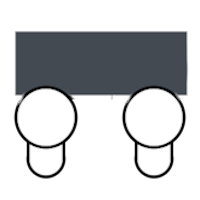
\includegraphics[height=7mm]{img/Icons/Attackers/Coffin.png}                  & \footnotesize{Coffin}                  & 0.4                 & 80               & \footnotesize{\textbf{Large.} \newline Spawns an \emph{Armored Skeleton} every 4s. \newline When killed, spawns 4 \emph{Skeletons}.}                \\
        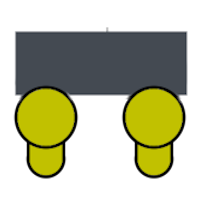
\includegraphics[height=7mm]{img/Icons/Attackers/Yellow Coffin.png}           & \footnotesize{Yellow Coffin}           & 0.4                 & 240              & \footnotesize{\textbf{Large.} \newline Spawns a \emph{Yellow Armored Skeleton} every 5s. \newline When killed, spawns 4 \emph{Yellow Skeletons}.}   \\
        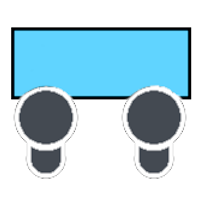
\includegraphics[height=7mm]{img/Icons/Attackers/Black Coffin.png}            & \footnotesize{Black Coffin}            & 0.4                 & 720              & \footnotesize{\textbf{Large.} \newline Spawns a \emph{Black Armored Skeleton} every 6s. \newline When killed, spawns 4 \emph{Black Skeletons}.}     \\
        
\includegraphics[height=7mm]{img/Icons/Attackers/Jellyfish.png}               & \footnotesize{Space Jellyfish}         & 0.8                 & 8                & \footnotesize{Takes 40\% less \emph{Physical} damage.}                                                                                              \\
        
\includegraphics[height=7mm]{img/Icons/Attackers/Blue Jellyfish.png}          & \footnotesize{Blue Space Jellyfish}    & 0.8                 & 40               & \footnotesize{Takes 50\% less \emph{Physical} damage.}                                                                                              \\
        
\includegraphics[height=7mm]{img/Icons/Attackers/Green Jellyfish.png}         & \footnotesize{Green Space Jellyfish}   & 0.8                 & 200              & \footnotesize{Takes 66\% less \emph{Physical} damage.}                                                                                              \\
        \bottomrule
    \end{tabular}
    \caption{The attacker types in the game (part 1).}
    \label{tab:attackers1}
\end{table}

\begin{table}[H]
    \centering
    \begin{tabular}{m{9mm}m{25mm}D{.}{.}{-1}rm{0.48\textwidth}}
        \toprule
        \textbf{Icon}                                                       & \textbf{Name}                & \mc{\textbf{Speed}} & \mc{\textbf{HP}} & \textbf{Description}                                                                                                                                        \\
        \midrule
        
\includegraphics[height=7mm]{img/Icons/Attackers/Fire Spirit.png}   & \footnotesize{Fire Spirit}   & 3                   & 6                & \footnotesize{Takes 50\% less \emph{Energy} damage.}                                                                                                        \\
        
\includegraphics[height=7mm]{img/Icons/Attackers/Forest Spirit.png} & \footnotesize{Forest Spirit} & 2                   & 15               & \footnotesize{Takes 66\% less \emph{Explosive} damage.}                                                                                                     \\
        
\includegraphics[height=7mm]{img/Icons/Attackers/Protector.png}     & \footnotesize{Protector}     & 1.4                 & 100              & \footnotesize{\textbf{Large.} \newline When killed, leaves behind a protective bubble 1.3 tiles in radius that blocks all projectiles from outside for 5s.} \\
        
\includegraphics[height=7mm]{img/Icons/Attackers/Druid.png}         & \footnotesize{Druid}         & 1                   & 120              & \footnotesize{\textbf{Large.} \newline Every 4s heals each attacker in a 1.6 tile radius by 15 HP.}                                                         \\
        \bottomrule
    \end{tabular}
    \caption{The attacker types in the game (part 2).}
    \label{tab:attackers2}
\end{table}


\begin{table}[H]
    \centering
    \begin{tabular}{m{15mm}m{20mm}lm{0.5\textwidth}}
        \toprule
        \textbf{Icon}                                                            & \textbf{Name}           & \textbf{Rarity} & \textbf{Description}                                                                             \\
        \midrule
        
\includegraphics[height=15mm]{img/Icons/Buildings/Dust Collector.png}    & Dust \newline Refinery  & Common          &
        \footnotesize{\textbf{Cost: 5 materials} \newline Produces 5 materials after every wave. \newline Cannot be placed on slants and adjacent to another Dust Refinery. \newline Increases cost by 5 materials when built.} \\

        
\includegraphics[height=15mm]{img/Icons/Buildings/Energy Harvester.png}  & Energy Harvester        & Rare            &
        \footnotesize{\textbf{Cost: 15 materials} \newline Whenever you gain Materials, produces 40\% as much Energy.}                                                                                                          \\

        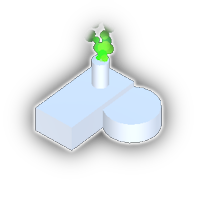
\includegraphics[height=15mm]{img/Icons/Buildings/Fuel Refinery.png}     & Fuel \newline Extractor & Rare            &
        \footnotesize{\textbf{Cost: 30 materials} \newline Cooldown 1 \newline Must be built on tiles rich in fuel. \newline Produces 10 fuel after every wave.}                                                                \\

        
\includegraphics[height=15mm]{img/Icons/Buildings/Matter Replicator.png} & Matter Replicator       & Rare            &
        \footnotesize{\textbf{Cost: 30 materials} \newline Cooldown 2 \newline Produces 5 materials after every wave, then increases its production by 5 materials.}                                                            \\

        
\includegraphics[height=15mm]{img/Icons/Buildings/Solar Panel.png}       & Solar Panel             & Common          &
        \footnotesize{\textbf{Cost: 5 materials} \newline Cannot be paced on slanted tiles. \newline The higher it's placed, the more energy it produces after every wave: 2 for every level of height.}                        \\

        
\includegraphics[height=15mm]{img/Icons/Buildings/Surface Drill.png}     & Surface Drill           & Starter         &
        \footnotesize{\textbf{Cost: 10 materials} \newline Must be built on tiles rich in minerals or fuel. \newline Produces 5 materials or 2 fuel after every wave.}                                                          \\
        \bottomrule
    \end{tabular}
    \caption{The economic building blueprints in the game.}
    \label{tab:economic-buildings}
\end{table}


\begin{table}[H]
    \centering
    \begin{tabular}{m{15mm}m{20mm}lm{0.5\textwidth}}
        \toprule
        \textbf{Icon}                                                          & \textbf{Name}      & \textbf{Rarity} & \textbf{Description}                                               \\
        \midrule
        
\includegraphics[height=15mm]{img/Icons/Buildings/Amplifier.png}       & Amplifier          & Legendary       &
        \footnotesize{\textbf{Cost: 40 materials} \newline Cooldown 2 \newline Range 2.3 \newline Increases damage of all towers in range by 3.}                                           \\

        
\includegraphics[height=15mm]{img/Icons/Towers/Frostbite Frontier.png} & Frostbite Frontier & Legendary       &
        \footnotesize{\textbf{Cost: 25 materials} \newline Range 2.1 \newline Freezes attackers in range, making them move 25\% slower and take 50\% more Energy damage.}                  \\

        
\includegraphics[height=15mm]{img/Icons/Buildings/Hub.png}             & Hub                & Special         &
        \footnotesize{Produces 10 fuel, 10 materials and 10 energy after every wave. \newline When an enemy reaches this building, you lose Hull, up to 5 per wave. Protect at all costs!} \\

        
\includegraphics[height=15mm]{img/Icons/Buildings/Radar.png}           & Radar              & Rare            &
        \footnotesize{\textbf{Cost: 10 materials} \newline Increases the range of adjacent buildings by 30\%.}                                                                             \\
        \bottomrule
    \end{tabular}
    \caption{The special building blueprints in the game.}
    \label{tab:special-buildings}
\end{table}


\begin{table}[H]
    \centering
    \begin{tabular}{m{15mm}m{20mm}lm{0.5\textwidth}}
        \toprule
        \textbf{Icon}                                                     & \textbf{Name} & \textbf{Rarity} & \textbf{Description}                                                                                                                                                                                                              \\
        \midrule
        
\includegraphics[height=15mm]{img/Icons/Towers/Budget Sentry.png} & Budget Sentry & Starter         &
        \footnotesize{\textbf{Cost: 10 materials} \newline Range 2.9 \newline Damage 2 (physical) \newline Interval 0.8s \newline Shoots projectiles at attackers in line of sight.}                                                                                                                                                            \\

        
\includegraphics[height=15mm]{img/Icons/Towers/Double Sentry.png} & Double Sentry & Common          &
        \footnotesize{\textbf{Cost: 15 materials} \newline Range 2.4 \newline Damage 2 (physical) \newline Interval 0.4s \newline Shoots projectiles at attackers in line of sight.}                                                                                                                                                            \\

        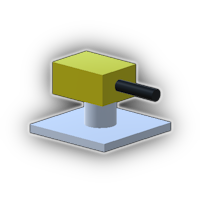
\includegraphics[height=15mm]{img/Icons/Towers/Galvanizer.png}    & Galvanizer    & Rare            &
        \footnotesize{\textbf{Cost: 10 energy 40 materials} \newline Range 3.7 \newline Damage 5 (physical) \newline Interval 0.5s \newline Shoots projectiles at attackers in line of sight. \newline When idle for 1.8s, charges up the next shot, making it deal additional 10 Energy damage and produce 5 energy when it hits an attacker.} \\

        
\includegraphics[height=15mm]{img/Icons/Towers/Gatling Gun.png}   & Gatling Gun   & Common          &
        \footnotesize{\textbf{Cost: 40 materials} \newline Range 3.3 \newline Damage 2 (physical) \newline Interval 0.15s \newline Needs to shoot continuously for 5s to spin up to maximum fire rate.}                                                                                                                                         \\
        \bottomrule
    \end{tabular}
    \caption{The tower blueprints in the game (part 1).}
    \label{tab:towers1}
\end{table}


\begin{table}[H]
    \centering
    \begin{tabular}{m{15mm}m{20mm}lm{0.5\textwidth}}
        \toprule
        \textbf{Icon}                                                      & \textbf{Name}  & \textbf{Rarity} & \textbf{Description}                                                                                                                                                                            \\
        \midrule
        
\includegraphics[height=15mm]{img/Icons/Towers/Mortar.png}         & Mortar         & Starter         &
        \footnotesize{\textbf{Cost: 25 materials} \newline Range 3.7 \newline Damage 4 (explosive) \newline Interval 2s \newline Cannot be paced on slanted tiles. \newline Shoots a cannonball over obstacles, impacting the ground after 1s and dealing damage to attackers within 1.2 tiles.}                \\

        
\includegraphics[height=15mm]{img/Icons/Towers/Predator.png}       & Predator       & Legendary       &
        \footnotesize{\textbf{Cost: 50 materials} \newline Range 3.4 \newline Damage 10 (physical) \newline Interval 1s \newline Shoots projectiles at attackers in line of sight. \newline Increases its damage by 1 with every kill.}                                                                         \\

        
\includegraphics[height=15mm]{img/Icons/Towers/Sledgehammer.png}   & Sledge-hammer  & Common          &
        \footnotesize{\textbf{Cost: 45 materials} \newline Range 1.6 \newline Damage 20 (explosive) \newline Interval 2.5s \newline Cannot be paced on slanted tiles. \newline Can be placed on tiles with small obstacles. \newline Smashes into the ground, dealing damage to all attackers in range.}        \\

        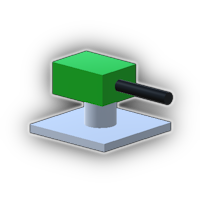
\includegraphics[height=15mm]{img/Icons/Towers/Sniper.png}         & Sniper         & Common          &
        \footnotesize{\textbf{Cost: 20 materials} \newline Range 11.1 \newline Damage 10 (physical) \newline Interval 3.3s \newline Shoots projectiles at attackers in line of sight. \newline The further away an attacker is, the more damage it takes, up to 200\%.}                                         \\

        
\includegraphics[height=15mm]{img/Icons/Towers/Static Sparker.png} & Static Sparker & Common          &
        \footnotesize{\textbf{Cost: 15 materials} \newline Range 3.3 \newline Damage 4 (energy) \newline Interval 1.9s \newline Hits its target, and then up to 3 more within 1.8 tiles from it, dealing half damage to each of them.}                                                                          \\

        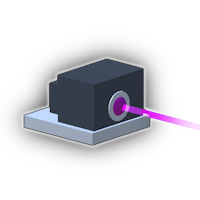
\includegraphics[height=15mm]{img/Icons/Towers/Ultra-Ray.png}      & Ultra-Ray      & Rare            &
        \footnotesize{\textbf{Cost: 30 materials} \newline Range 8.1 \newline Damage 1 (energy) \newline Interval 0.15s \newline Press [R] to rotate. \newline Can be placed on tiles with small obstacles. \newline Fires a continuous beam in a fixed cardinal direction, hitting up to 5 attackers at once.} \\
        \bottomrule
    \end{tabular}
    \caption{The tower blueprints in the game (part 2).}
    \label{tab:towers2}
\end{table}


\begin{table}[H]
    \centering
    \begin{tabular}{m{15mm}m{20mm}lm{0.5\textwidth}}
        \toprule
        \textbf{Icon}                                                          & \textbf{Name}   & \textbf{Rarity} & \textbf{Description}                                                                                                                                                                                                                                                  \\
        \midrule
        
\includegraphics[height=15mm]{img/Icons/Abilities/Catalyst.png}        & Catalyst        & Rare            &
        \footnotesize{\textbf{Cost: 20 energy} \newline Cooldown 1 \newline Radius 0.8 \newline Afflicts attackers within radius, making them take 2x as much damage and produce 1 Material when killed.}                                                                                                                                                                                  \\

        
\includegraphics[height=15mm]{img/Icons/Abilities/Grenade.png}         & Grenade         & Starter         &
        \footnotesize{\textbf{Cost: 10 energy} \newline Radius 0.75 \newline Damage 4 (explosive) \newline Deals damage to all attackers within radius.}                                                                                                                                                                                                                                   \\

        
\includegraphics[height=15mm]{img/Icons/Abilities/HoloSiphon.png}      & Holo-Siphon     & Rare            &
        \footnotesize{\textbf{Cost: 10 energy} \newline Cooldown 1 \newline Range 2.4 \newline Damage 3 (HP loss) \newline Interval 1.5s \newline Can be placed on tiles with small obstacles. \newline When placed, instantly deals damage to all attackers within range. \newline Conjures a tower for 3 waves. Attacker targeted by it must stay within range for 1.2s to take damage.} \\

        
\includegraphics[height=15mm]{img/Icons/Abilities/Lightning Storm.png} & Lightning Storm & Common          &
        \footnotesize{\textbf{Cost: 15 energy} \newline Radius 2.5 \newline Damage 25 (energy) \newline Interval 1s \newline Strikes 6 times, each time hitting a random attacker within radius.}                                                                                                                                                                                          \\

        \includegraphics[height=15mm]{img/Icons/Abilities/Meteor.png}          & Meteor          & Common          &
        \footnotesize{\textbf{Cost: 25 energy} \newline Radius 1.4 \newline Damage 16 (physical and explosive) \newline Impacts the ground after 0.8s, dealing damage to all attackers within radius.}                                                                                                                                                                                     \\

        \includegraphics[height=15mm]{img/Icons/Abilities/Orbital Laser.png}   & Orbital Laser   & Rare            &
        \footnotesize{\textbf{Cost: 30 energy} \newline Damage 30 (energy) \newline Duration 3s \newline Press [R] to rotate. \newline Sweeps across the world in a cardinal direction, dealing damage to each attacker in its path.}                                                                                                                                                      \\

        \includegraphics[height=15mm]{img/Icons/Abilities/Streamline.png}      & Streamline      & Legendary       &
        \footnotesize{\textbf{Cost: 10 energy 10 materials} \newline Cooldown 1  \newline Improves other blueprints for the rest of the battle: \newline Makes them 2 materials cheaper. \newline Increases Range and Radius by 5\%. \newline Decreases Interval by 10\%, to a minimum of 0.25s.}                                                                                          \\
        \bottomrule
    \end{tabular}
    \caption{The ability blueprints in the game.}
    \label{tab:abilities}
\end{table}
